\documentclass[11pt]{article}
\usepackage{c://pctex/activity}

\lhead{}
\chead{\textbf{\large{Exercise 11 - Section 9.3\\The Closed Interval $\boldsymbol{\left[ 0, 1 \right]}$}}}
\rhead{}
\lfoot{\emph{Mathematical Reasoning: Writing and Proof, Third Ed.} \\Ted Sundstrom}
\cfoot{}
\rfoot{\copyright \the\year\, by Pearson Education, Inc.\\}


\begin{document}
\begin{enumerate}
\item Let $f: \left[ 0, 1 \right] \to \left[ 0, 1 \right)$ by
\begin{equation} \notag
f \left( x \right) = 
\begin{cases}
\dfrac{1}{n+1}         &\text{if $x=\dfrac{1}{n}$ for some $n \in \mathbb{N}$} \\
 %                     &                      \\
x        &\text{otherwise}
\end{cases}
\end{equation}
\begin{enumerate}
\item 
$f \left( 0 \right) = 0$,
$f \left( 1 \right) = \dfrac{1}{2}$, 
$f \left( \dfrac{1}{2} \right) = \dfrac{1}{3}$, 
$f \left( \dfrac{1}{3} \right) = \dfrac{1}{4}$, 
$f \left( \dfrac{1}{4} \right) = \dfrac{1}{5}$,
$f \left( \dfrac{1}{5} \right) = \dfrac{1}{6}$.

\item The graph below shows some of the graph of the function $f$.  The points marked with a small square on the line $y = x$ indicate the points that have been removed from this line.  They have been replaced by the points marked with a small circle.  The graph shows 6 points that have been removed and the 6 points that have replaced them.  The process continues, but this is not shown on the graph.
%
\begin{center}
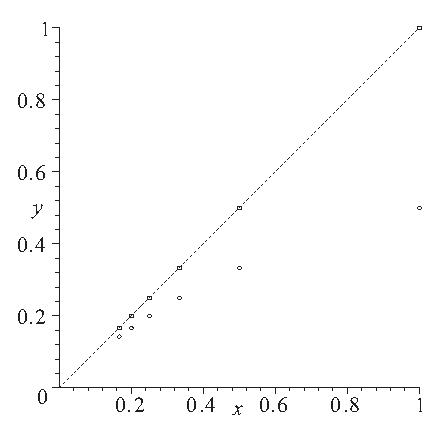
\includegraphics{figps-sec93-1.eps}
\end{center}
%
\item From the graph, we see that function $f$ is an injection.  We also see that the range of 
$f$ is the interval $\left[ 0, 1 \right)$, and hence, $f$ is a surjection.  

\item Since $f$ is a bijection, we conclude that $\left[0, 1 \right] \approx \left[ 0, 1 \right)$.
\end{enumerate}

\newpage
\item Let $g: \left[ 0, 1 \right) \to \left( 0, 1 \right)$ by
\begin{equation} \notag
g \left( x \right) = 
\begin{cases}
\dfrac{1}{2}           &\text{if $x=0$} \\
%                      &                      \\
\dfrac{1}{n+1}         &\text{if $x=\dfrac{1}{n}$ for some $n \in \mathbb{N}$} \\
%                      &                      \\
x        &\text{otherwise}
\end{cases}
\end{equation}
%
\begin{enumerate}
\item The following graph shows some of the graph of the function $g$.  The points marked with a small square on the line $y = x$ indicate the points that have been removed from this line.  They have been replaced by the points marked with a small circle.  The graph shows 6 points that have been removed and the 6 points that have replaced them.  The process continues, but this is not shown on the graph.  Notice that the point $\left( 0, \dfrac{1}{2} \right)$ has been added, and there is no point on the graph with $x = 1$ since 1 is not in the domain of $g$.

\begin{center}
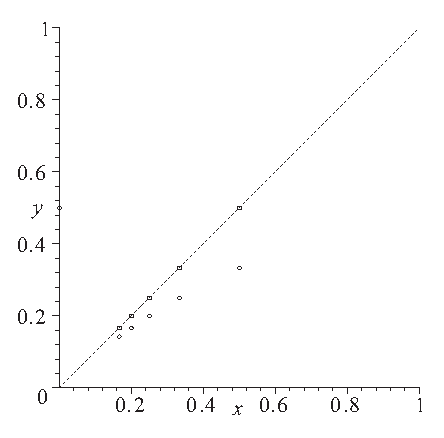
\includegraphics{figps-sec93-2.eps}
\end{center}
%
\item From the graph, we see that function $g$ is an injection.  We also see that the range of 
$g$ is the open interval $\left( 0, 1 \right)$, and hence, $g$ is a surjection.  

\item Since $g$ is a bijection, we conclude that $\left[0, 1 \right) \approx \left( 0, 1 \right)$.
\end{enumerate}

\item Part~(1) and Part~(2) show that the intervals $\left[0, 1 \right]$, $\left[0, 1 \right)$, and $\left(0, 1 \right)$ are all equivalent.  Therefore, each of the intervals is uncountable and has cardinality $\boldsymbol{c}$.


\end{enumerate}

\end{document}
